    \documentclass{article}
%------------------------- packages -------------------------%
\usepackage[vietnamese.licr]{babel}
\usepackage{listings}
\usepackage{tvietlistings}
\usepackage[T1]{fontenc}
\usepackage[utf8]{inputenc} % Đảm bảo sử dụng mã hóa UTF-8
\usepackage{float}
\usepackage[many]{tcolorbox}
\usepackage[unicode,hidelinks]{hyperref}    % for reference
\usepackage{geometry}   % for layout
\usepackage{amsmath}    % for math
\usepackage{xcolor}     % for color
% for figure
\usepackage{graphicx}
\usepackage{caption}    
% for code
\usepackage{minted}
\usepackage[normalem]{ulem}
% for table
\usepackage{xparse}
\usepackage{float}      
\usepackage{paracol}
\usepackage{array}
\usepackage{multirow}
% for header & footer 
\usepackage{fancyhdr}
\usepackage{lastpage}
\usepackage{CJKutf8}
\usepackage{xcolor}


%------------------------- set up -------------------------%
% figure
\graphicspath{{./Images/}}              % path to image
\captionsetup[figure]{labelfont={small,bf,it},textfont={small,it}}
% paragraph
\setlength{\parindent}{0pt}
\setlength{\parskip}{12pt}
\setlength{\parskip}{6pt}               % disables indentation
\renewcommand{\baselinestretch}{1.5}    % line spacing

% code
\def\code#1{\texttt{#1}}    % font
\usemintedstyle{vs}         % minted theme
\setminted{
    autogobble,             % remove all common leading whitespace
    baselinestretch=1.0,
    bgcolor=gray!5!white,
    breaklines,
    %linenos,               % enables line numbers
    fontsize=\footnotesize
}
% Table addrow Macro with dyanamic
% Define the new addrow command to accept a variable number of arguments
\NewDocumentCommand{\addrow}{>{\SplitList{;}}m}{%
  \processline#1\relax
}


% Define a custom style
\lstdefinestyle{myStyle}{
    frame=l,
    framesep=4.5mm,
    framexleftmargin=2.5mm,
    basicstyle=\ttfamily\footnotesize,
    captionpos=b,
    commentstyle=\color{comment},
    breakatwhitespace=false,         
    breaklines=true,                 
    keepspaces=true,                 
    numbers=left,       
    numbersep=5pt,                  
    showspaces=false,                
    showstringspaces=false,
    showtabs=false,                  
    tabsize=2,
    keywords={if, else, for, while, repeat, function, in, next, break, library, ifelse, select, return, print, mutate, hist, tapply, apply, sapply, boxplot, barplot, factor},
		% keywordstyle=\color{blue}\bfseries,
        keywordstyle=\color{comment},
		ndkeywords={class, data.frame, numeric, matrix, character, list, c, seq},
		ndkeywordstyle=\color{black}\bfseries,
		identifierstyle=\color{black},
		sensitive=false,
		comment=[l]{\#},
}
% Helper macro to process each item
\newcommand{\processline}[1]{%
  \ifx\relax#1\relax % End of the list
    \\ \hline
  \else
    #1%
    \expandafter\processnext
  \fi
}

\newcommand{\processnext}[1]{%
  \ifx\relax#1\relax % End of the list
    \\ \hline
  \else
    & #1%
    \expandafter\processnext
  \fi
}

% Callout
\definecolor{main}{HTML}{5989cf}    % setting main color to be used
\definecolor{comment}{HTML}{606060}
\definecolor{sub}{HTML}{cde4ff}     % setting sub color to be used
\newtcolorbox{boxH}{
    % fontupper = \bf,
    boxrule = 1.5pt,
    colback = white, 
    colframe = black % frame color
}
% End
%------------------------- layout & margin -------------------------%
\geometry{
    a4paper,        % redundant if already in \documentclass
    left=20.32mm,
    right=20.32mm,
    top=25.40mm,
    bottom=25.40mm,
    heightrounded,  % better use it
}
\setlength{\parindent}{20pt}
%------------------------- header & footer -------------------------%
\renewcommand{\headrulewidth}{0.5pt}
\renewcommand{\footrulewidth}{0.5pt}
\setlength{\headheight}{24.5pt}
\pagestyle{fancy}

\fancyhead{}    % clear all header fields
\fancyhead[L]{
    \begin{tabular}{ll}
        \begin{picture}(10,10)
            \put(0,-7){
\includegraphics[width=8mm]{{Images/bachkhoa_logo.png}}}
        \end{picture}&
    	\begin{tabular}{l}
    	    {\ttfamily Trường Đại học Bách Khoa Tp. Hồ Chí Minh} \\
    	    {\ttfamily Khoa Khoa học và Kỹ thuật Máy tính} \\
    	\end{tabular} 	
    \end{tabular}
}

\fancyfoot{}    % clear all footer fields
\fancyfoot[L]{\footnotesize {\ttfamily Báo cáo bài tập lớn Lập trình nâng cao Kì 241}}
\fancyfoot[R]{\footnotesize {\ttfamily Trang {\thepage}/\pageref{LastPage}}}
% might change to \scriptsize

%------------------------- body -------------------------%
\begin{document}


% Use \lstset to make myStyle the global default
\lstset{style=myStyle}
%-------------------- cover --------------------%
\begin{titlepage}
\begin{center}
    \large ĐẠI HỌC QUỐC GIA THÀNH PHỐ HỒ CHÍ MINH \\
    TRƯỜNG ĐẠI HỌC BÁCH KHOA \\
    KHOA KHOA HỌC VÀ KỸ THUẬT MÁY TÍNH
\end{center}

\vspace{1.5cm}

\begin{figure}[!ht]
    \centering 
\includegraphics[width=3.5cm]{Images/bachkhoa_logo.png}
\end{figure}

\vspace{1.5cm}

\begin{table}[H]
    \centering
    \begin{tabular}{c}
    {\bf \Large Lập Trình Nâng Cao (MT2013)} \\ \\
    \hline  \\
    \multicolumn{c}{c}{{\bf \huge Báo cáo Bài tập lớn}}    \\  \\
    {\bf CHƯƠNG TRÌNH THỐNG KÊ CHUYỂN KHOẢN CHO MTTQ}     \\  
    {\bf  TỪ NGÀY 01/09/2024 ĐẾN NGÀY 11/09/2024}     \\  \\
    \hline
    \end{tabular}
\end{table}

\vspace{1.5cm}

\begin{table}[h]
\centering
\begin{tabular}{lrlc}

\hspace{0 cm} & GVHD: THẦY LÊ ĐÌNH THUẬN  & \vspace{0.5cm}\\
& Các thành viên nhóm \textbf{504} gồm: &  
 	
    Bùi Nguyễn Hoàng Thọ& 2333017\\
& & Đặng Minh Quân & 2212775\\
& & Nguyễn Trung Phú& 2212592\\
& & Tôn Viết Trí & 2213603\\
& & Nguyễn Như Thắng & 2213203\\
\end{tabular}
\textbf{\textit{}}\end{table}

\vspace{1.0cm}

\begin{center}
    \footnotesize Tp. Hồ Chí Minh, Tháng 12/2024
\end{center}
\end{titlepage}
\newpage
\begin{table}[H]
\centering
\resizebox{\textwidth}{!}{
\begin{tabular}{|l|l|p{10cm}|}
\hline
\textbf{TÊN SINH VIÊN} & \textbf{MÃ SỐ SINH VIÊN} & \textbf{MÔ TẢ CÔNG VIỆC} \\ 
\hline
Bùi Nguyễn Hoàng Thọ   & 2333017                 & Kiểm định lại sản phẩm và viết báo cáo bằng latex \\ 
\hline
Đặng Minh Quân          & 2212775                 & Thiết kế giao diện người dùng và kết quả hiện thị. 
 \\ 
\hline
Nguyễn Trung Phú        & 2212592                 & Chuyển dữ liệu từ CSV sang Json, thiết kế slide báo cáo \\ 
\hline
Tôn Viết Trí         & 2213603                 & Viết hàm KMP phục vụ tìm kiếm kết quả và phân trang\\ 
\hline
Nguyễn Như Thắng       & 2213203                 & Lên ý tưởng thiết kế giao diện. Thực hiện slide báo cáo.\\ 
\hline
\end{tabular}
}
\caption{Bảng mô tả đóng góp từng thành viên nhóm 504}
\label{tab:motadonggoptungthanhvien}
\end{table}

\newpage
%-------------------- mission --------------------%
%\renewcommand{\arraystretch}{2}

%-------------------- mục lục --------------------%
\tableofcontents
%-------------------- Chia các mục --------------------%
\section*{\begin{center}
\Huge{Giới thiệu}
\end{center}}
Trong thời gian vừa qua, đất nước chúng ta đã chịu ảnh hưởng nặng nề từ cơn bão Yagi, gây ra những thiệt hại không thể đong đếm. Phát huy tinh thần \textit{lá lành đùm lá rách} của dân tộc, Mặt Trận Tổ Quốc Việt Nam đã tổ chức phong trào quyên góp để hỗ trợ đồng bào bị ảnh hưởng, giúp khôi phục đời sống hàng ngày.

Nhằm cung cấp một công cụ tìm kiếm thông tin nhanh chóng và tiện lợi, dự án web app \textbf{"Thống kê chuyển khoản"} đã ra đời. Sản phẩm này được thiết kế với giao diện đơn giản, thân thiện với người dùng.

Báo cáo dưới đây là kết quả nghiên cứu và thực hiện của nhóm 504 trong khuôn khổ môn \textit{Lập trình nâng cao}.

\section{Tổng quan}
\subsection{Yêu cầu}
\begin{itemize}
\item Quá trình tìm kiếm phải nhanh, đảm bảo độ chính xác cao nhất.
\item Dữ liệu phải đầy đủ, chính xác, không chứa ký tự lạ hoặc lỗi.
\item Thao tác tra cứu phải đơn giản và thuận tiện.
\end{itemize}

\subsection{Kết quả mong muốn}
\begin{itemize}
\item Kết quả hiển thị dưới dạng bảng.
\item Phân trang đầy đủ.
\item Có thể sắp xếp (\textit{sort}) dữ liệu theo ngày hoặc giá tiền.
\item Các trường dữ liệu phải được hiển thị đầy đủ: \textbf{Chi tiết tin nhắn (\textit{detail})}, \textbf{tiền chuyển khoản (\textit{credit})}, \textbf{tiền trừ (\textit{debit})}, \textbf{ngày giao dịch (\textit{date})}.
\end{itemize}

\subsection{Thuật toán sử dụng}
Sau khi nghiên cứu các thuật toán tìm kiếm khả thi, nhóm quyết định áp dụng thuật toán \textbf{Knuth-Morris-Pratt (KMP)} nhằm tối ưu hóa hiệu suất.

\subsection{Ngôn ngữ lập trình}
Nhóm chia dự án thành hai phần: \textit{frontend} và \textit{backend}.
\begin{itemize}
\item \textbf{Frontend}: Sử dụng \textbf{HTML}, \textbf{CSS} để thiết kế giao diện.
\item \textbf{Backend}: Dùng \textbf{Express} để tạo API kết nối dữ liệu mẫu và \textbf{JavaScript} để mô phỏng thuật toán \textbf{KMP} cùng các tính năng khác như \textit{sort} (sắp xếp).
\end{itemize}

\section{Thuật toán KMP}
\subsection{Định nghĩa}
Thuật toán Knuth-Morris-Pratt (KMP) là một phương pháp tìm kiếm chuỗi đầu vào (\textit{pattern}) trong một chuỗi cho trước (\textit{text}) trong thời gian tuyến tính. Thuật toán khai thác các tiền tố (\textit{prefix}) và hậu tố (\textit{suffix}) của chuỗi con để bỏ qua những phần không cần so sánh, giúp tăng hiệu quả xử lý.

\subsection{Ý tưởng chính}
KMP dựa trên nguyên tắc rằng nếu một phần chuỗi đã khớp, ta có thể tận dụng thông tin này để tiếp tục tìm kiếm thay vì so sánh lại từ đầu. Thuật toán tính trước một bảng \textit{hàm tiền tố} (\textit{prefix function}), xác định vị trí so sánh tiếp theo khi không khớp.

\subsection{Các bước thực hiện}
\begin{itemize}
\item \textbf{Bước 1: Xây dựng bảng tiền tố}. Trước khi tìm kiếm, thuật toán tính bảng tiền tố cho chuỗi cần tìm, làm cơ sở cho các thao tác bước sau.
\item \textbf{Bước 2: Tìm kiếm}. Dùng bảng tiền tố để xác định phần tiếp theo cần so sánh khi không khớp, tiết kiệm thời gian.
\end{itemize}

\begin{figure}[!hbt]
\centering 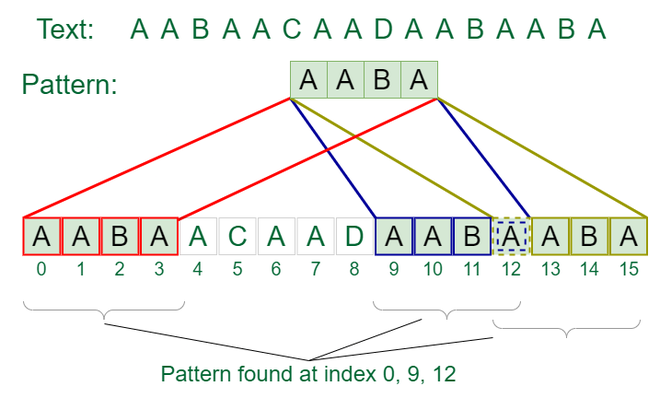
\includegraphics[width=15cm]{Images/img/kmp.png}
\caption{Minh họa thuật toán KMP}
\end{figure}
\newpage
\section{Cấu trúc dữ liệu}
\subsection{Dữ liệu}
Nhóm quyết định sử dụng \textbf{JSON} thay vì \textbf{CSV} nhằm tăng tính linh hoạt trong quá trình xử lý.

\begin{figure}[!ht]
\centering 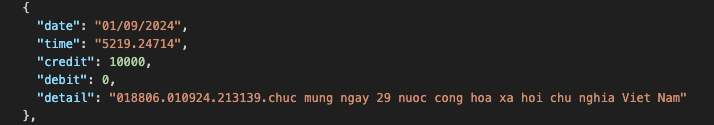
\includegraphics[width=15cm]{Images/img/json.png}
\caption{Cấu trúc dữ liệu JSON}
\end{figure}

\begin{itemize}
\item \textbf{date}: Ngày chuyển khoản
\item \textbf{time}: Thời gian chuyển khoản
\item \textbf{credit}: Tiền chuyển khoản
\item \textbf{debit}: Tiền trừ
\item \textbf{detail}: Tin nhắn chuyển tiền
\end{itemize}

\subsection{Frontend}
\begin{itemize}
\item \textbf{index.html}: Chứa giao diện trang web.
\item \textbf{decor.css}: Quản lý giao diện và hiểu ứng thị giác.
\item \textbf{script.js}: Xử lý chức năng giao diện, kết nối API.
\end{itemize}

\subsection{Backend}
Phần \textit{backend} đảm nhận vai trò tạo API truy vấn dữ liệu từ các tệp JSON, hiển thị thông tin trên trang web.
\begin{itemize}
    \item \textbf{Server.js}: Thực hiện việc tạo api truy vấn các dữ liệu trong \textbf{data.json} và thực hiện thuật toán KMP.
\end{itemize}
\subsection{Thư viện và công cụ}
\begin{itemize}
    \item \textbf{Axios}: kết nối đến API và trả về kết quả cho frontend
    \item \textbf{fs}: Đọc files từ local.
\end{itemize}  

\section{Cách thức hoạt động}
\subsection{Backend}
\subsubsection{Đọc dữ liệu từ tệp JSON}
Server đọc dữ liệu từ tệp \texttt{data.json} bằng cách:
\begin{itemize}
    \item Xác định đường dẫn của tệp: \texttt{path.join(\_\_dirname, 'data', 'data.json')}.
    \item Đọc nội dung tệp với mã hóa \texttt{'utf-8'} bằng hàm \texttt{fs.readFileSync}.
    \item Chuyển đổi dữ liệu từ định dạng chuỗi sang đối tượng JSON bằng \texttt{JSON.parse}.
\end{itemize}

\subsubsection{Xử lý thuật toán Knuth-Morris-Pratt (KMP)}
\begin{itemize}
    \item \textbf{Xây dựng bảng tiền tố (LPS)}:
    \begin{itemize}
        \item Tạo một mảng \texttt{lps} để lưu trữ độ dài các tiền tố trùng khớp.
        \item Duyệt qua chuỗi \texttt{pattern}, tính toán các giá trị trong bảng \texttt{lps}.
    \end{itemize}
    \item \textbf{Tìm kiếm chuỗi}:
    \begin{itemize}
        \item Dựa vào bảng \texttt{lps}, so sánh các ký tự trong \texttt{pattern} và \texttt{text}.
        \item Khi phát hiện không khớp, sử dụng bảng \texttt{lps} để bỏ qua các so sánh không cần thiết.
        \item Trả về kết quả khi tìm thấy hoặc không tìm thấy chuỗi.
    \end{itemize}
\end{itemize}

\subsubsection{Xử lý API tìm kiếm}
\begin{itemize}
    \item Endpoint \texttt{/api/data} nhận tham số \texttt{term} từ truy vấn người dùng.
    \item Chuyển đổi chuỗi tìm kiếm sang chữ thường (\texttt{toLowerCase}) để so sánh không phân biệt chữ hoa/thường.
    \item Lọc dữ liệu JSON dựa trên thuật toán KMP:
    \begin{itemize}
        \item Tìm kiếm \texttt{term} trong trường \texttt{detail} của từng mục dữ liệu.
        \item Chỉ trả về những mục có chứa chuỗi khớp.
    \end{itemize}
    \item Kết quả được trả về dưới dạng JSON.

\begin{figure}[!ht]
\centering
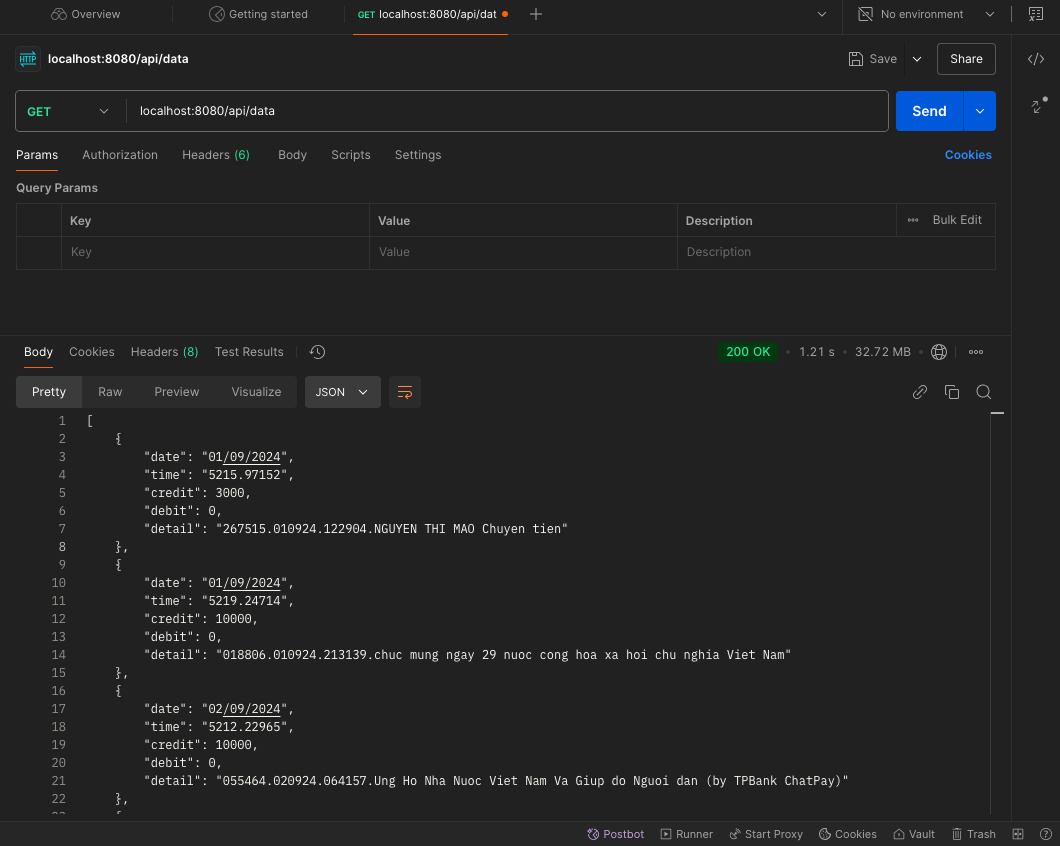
\includegraphics[width=15cm]{Images/img/postman.png}
\caption{Trong postman}
\end{figure}
\end{itemize}
\subsection{Frontend}
\begin{enumerate}
    \item \textbf{Quản lý dữ liệu và phân trang:}
    \begin{itemize}
        \item Mảng \texttt{allData} được sử dụng để lưu trữ toàn bộ dữ liệu từ API.
        \item Các biến \texttt{currentPage} và \texttt{resultsPerPage} điều chỉnh số lượng kết quả hiển thị trên mỗi trang.
        \item Hàm \texttt{renderTable} hiển thị dữ liệu theo từng trang, kết hợp với \texttt{renderPagination} để tạo giao diện phân trang.
    \end{itemize}

    \item \textbf{Xử lý API và debounce:}
    \begin{itemize}
        \item Hàm \texttt{performSearch} gọi API với tham số tìm kiếm, lưu kết quả vào \texttt{allData}, và cập nhật giao diện bảng.
        \item Sử dụng cơ chế debounce để giảm tải các yêu cầu API khi người dùng nhập liệu liên tục.
    \end{itemize}

    \item \textbf{Định dạng và tính toán dữ liệu:}
    \begin{itemize}
        \item Hàm \texttt{updateTotalAmount} tính tổng chênh lệch giữa \texttt{credit} và \texttt{debit} để hiển thị tổng thu.
    \end{itemize}

    \item \textbf{Sắp xếp và lọc dữ liệu:}
    \begin{itemize}
        \item Hàm \texttt{sortTableByDate} sắp xếp dữ liệu theo ngày giao dịch, \texttt{sortTableByAmount} sắp xếp theo số tiền (tăng hoặc giảm dần).
        \item Hàm \texttt{searchByTerm} lọc dữ liệu dựa trên từ khóa tìm kiếm.
    \end{itemize}

    \item \textbf{Giao diện và tương tác:}
    \begin{itemize}
        \item Hàm \texttt{toggleFilterMenu} mở hoặc đóng menu bộ lọc.
        \item Hiển thị thông báo khi không tìm thấy kết quả hoặc khi xảy ra lỗi tải dữ liệu.
    \end{itemize}
\end{enumerate}

\section{Giao diện chương trình và đánh giá}
\subsection{Chạy server}
Khởi động server để chương trình để lấy dữ liệu. 
\begin{lstlisting}[language=bash, caption=Khởi động server]
npm install # Cài đặt các thư viện cân thiết
npm start # Khởi động server

\end{lstlisting}


\begin{lstlisting}[language=bash,caption="Server đã chạy thành công"]
thohnb@192 hcmut-ltnc-assigment % npm start
> be@1.0.0 start
> node server.js
Server is running on http://localhost:8080
\end{lstlisting}

\subsection{Giao diện chính}
\begin{figure}[!ht]
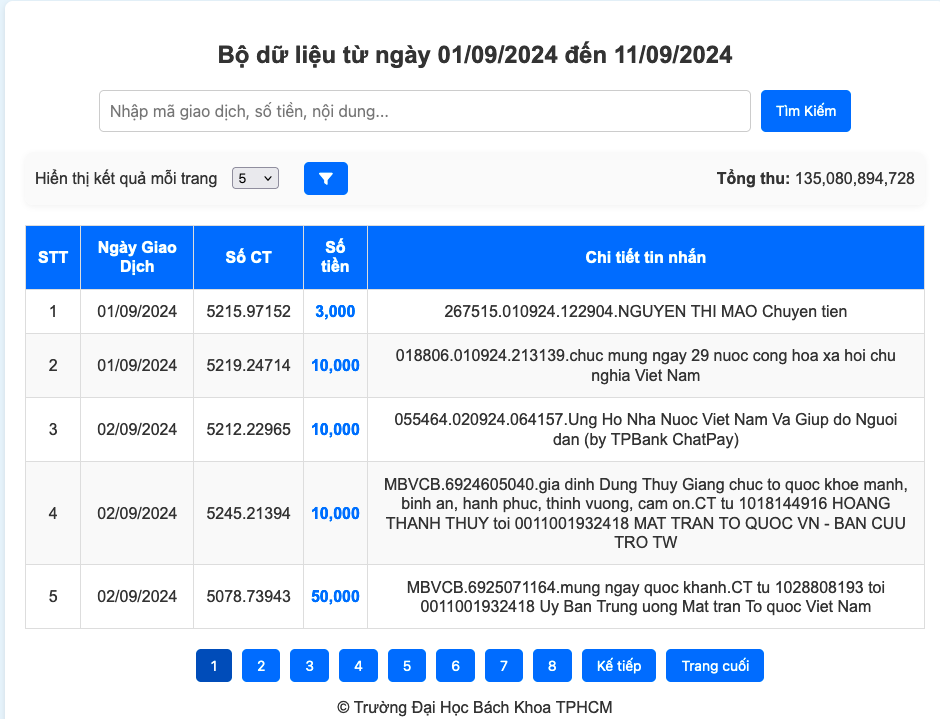
\includegraphics[width=15cm]{Images/img/main_screen_2.png}
\caption{Giao diện chính}
\end{figure}
\newpage
Nhập kết quả và xuất ra dữ liệu tìm thấy dưới dạng bảng

\begin{figure}[!ht]
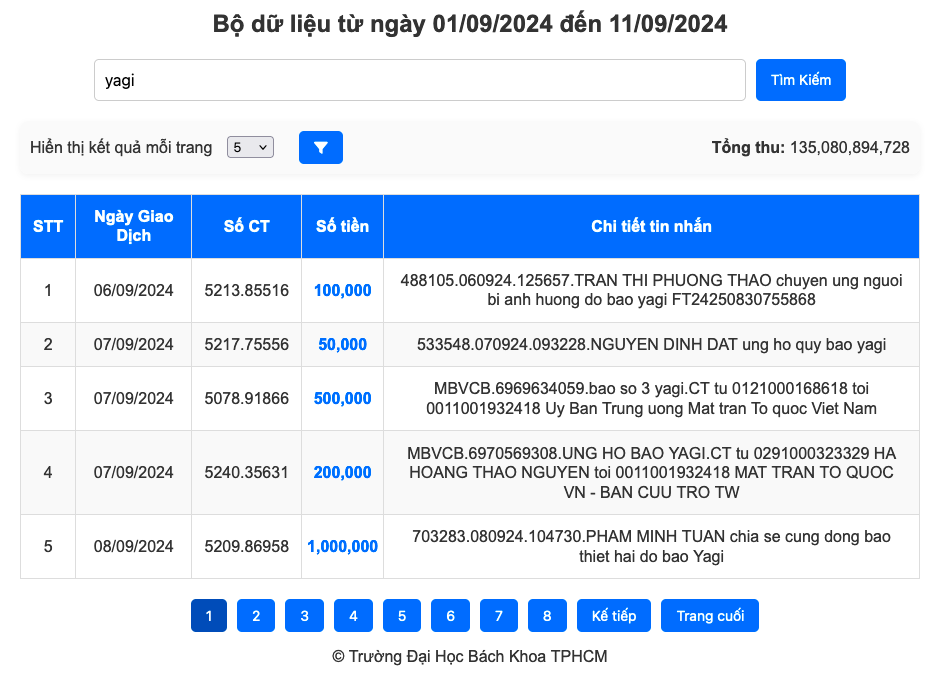
\includegraphics[width=15cm]{Images/img/searching.png}
\caption{Xuất kết quả tìm kiếm}
\end{figure}


\begin{figure}[!ht]
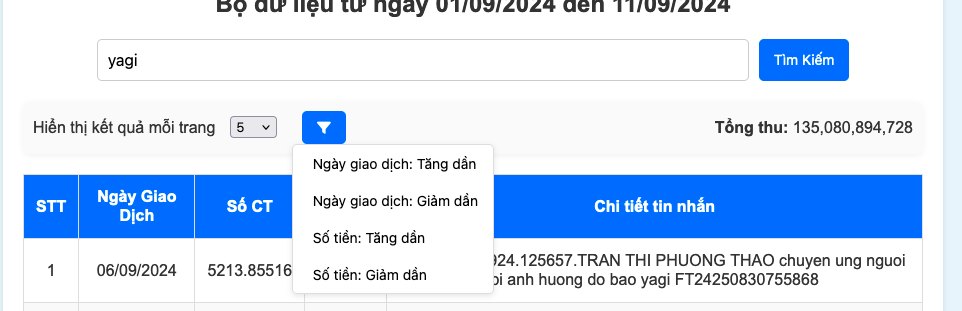
\includegraphics[width=15cm]{Images/img/filter_and_show_result_per_page.png}
\caption{Sắp xếp và số lượng kết quả mỗi trang}
\end{figure}
\newpage
Khi người dùng chọn lọc kết quả theo giá tiền/ ngày tháng từ thấp đến cao.
\begin{figure}[!ht]
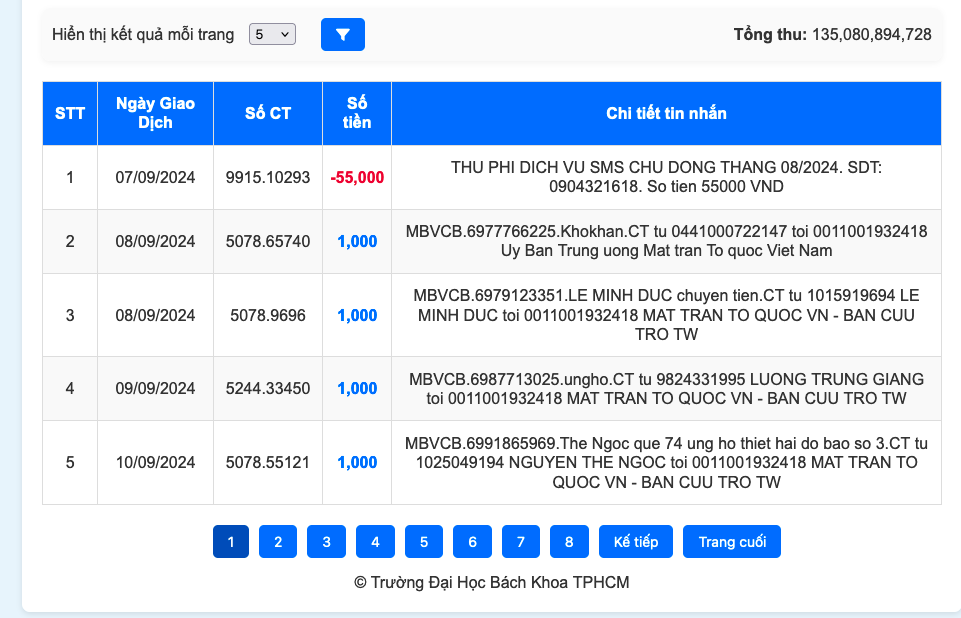
\includegraphics[width=15cm]{Images/img/order_lowest_to_hhighest_credit.png}
\caption{Sắp xếp và số lượng kết quả mỗi trang}
\end{figure}
\section{Kết luận và khả năng mở rộng}
Như vậy, qua những nội dung nhóm đã đề cập ở trên, nhóm xin được rút ra những gì nhóm đã làm được và những điểm hạn nhóm cần khắc phục.

\subsection{Đã làm được}
\begin{itemize}
    \item Hệ thống hoàn thiện, ổn định 
    \item Hiện thị kết quả rõ ràng
    \item Giao diện thể hiện trực quan.
\end{itemize}

\subsection{Hạn chế}
\begin{itemize}
    \item Hệ thống còn đơn giản , còn nhiều thứ nhóm chưa làm được những thứ phức tạp hơn như lấy tên họ người gửi
\item Tốc độ còn chậm, chưa được tối ưu hóa nhiều
\item Chưa làm được tính năng tính tổng thu (lấy toàn bộ giá trị \textbf{credjt} có trong json.
\item Chưa tìm kiếm được theo giá trị. Chỉ tìm kiếm được trong phạm vi tin nhắn chuyển khoản.
\end{itemize}


\section{Tài liệu tham khảo}
\begin{itemize}
    \item Thuật toán KMP : https://wiki.vnoi.info/translate/wcipeg/kmp
    \item Xử lý string: https://wiki.vnoi.info/algo/string/basic
\end{itemize}

\textbf{Source Code Bài tập lớn}: https://github.com/bnhtho/hcmut-ltnc-assigment 
%-------------------- main --------------------%
\phantomsection

% --------- Document Note --------------
% ╔═══════════════════════╗
% ║       Table           ║
% ╚═══════════════════════╝
% \begin{table}[H]
% \begin{tabular}{|l|r|c|c|} % Define how many columns of table[1]
% \hline
% Use \addrow to create new row % Need equal columns number that define in [1] and seprate by ;
% \addrow {<columns-data>;<columns-data2>...};
% \end{tabular}
% \end{table}
% ╔═══════════════════════╗
% ║       Math Equation   ║
% ╚═══════════════════════╝
% Inline Equation: use $<formula>$
% For Block Equation: use $$ <formula> $$
% ╔═══════════════════════╗
% ║       Coding          ║
% ╚═══════════════════════╝
% \begin{lstlisting}[language=R, caption=<Example Caption>]
% -- Start your code
% \end{lstlisting}

\end{document}

